\documentclass[12pt]{scrartcl}
\title{Assignment 3\\ Design Thinking:\\ Sketches and Wireframes}
\author{\textbf{Flow Overstack Team}\\ Cesana Filippo\\ Hartmann Kathrin\\ Gary\\ Rodolfo Masera Tommaso\\ Stucchi Jacopo\\ Taillefert Stefano}
\date{}
\setlength{\parindent}{0pt}

\usepackage{graphicx}
\usepackage{float}

\begin{document}

\maketitle

\tableofcontents

\newpage


\section{Introduction}

	Write a brief introduction referring back to your project and it basic concepts.

\section{Persona}

	% Describe briefly your design persona as distilled from the analysis of data gathered during Contextual Inquiry.
	
	The first task we went through was to summarize the interviews we conducted and extract meaningful data from all the kids' 
	answers, to construct a user model for our application. The result is Kiddo, our design persona.\\
	
	Kiddo is the average 12-years-old, goes to middle school and loves spending time on his smartphone. He uses it mainly for 
	entertainment purposes, following his favorite youtubers and idols on social media, listening to music and chat with his on- 
	and offline friends.\\
	
	His inspirations are people like Footballo Socceri, the famous football player who always trash-talks his opponents on Twitter; 
	Trappino Trappisti, a rapper who rose to fame after punching a child on the street and whose songs are mainly violence-themed;
	Thotella DeThot, a TV showgirl widely known for her osé selfies posted on Instagram; and many others.\\
	
	He doesn't dislike school, but he finds the ``classic" way of studying quite boring, bent over a textbook trying to memorize 
	dates and facts that he will forget in a couple of days anyway. In class, he often dreams of being somewhere else, learning 
	something that he is \textit{really} interested in.
	
	\begin{figure}[H]
        		\centering
       		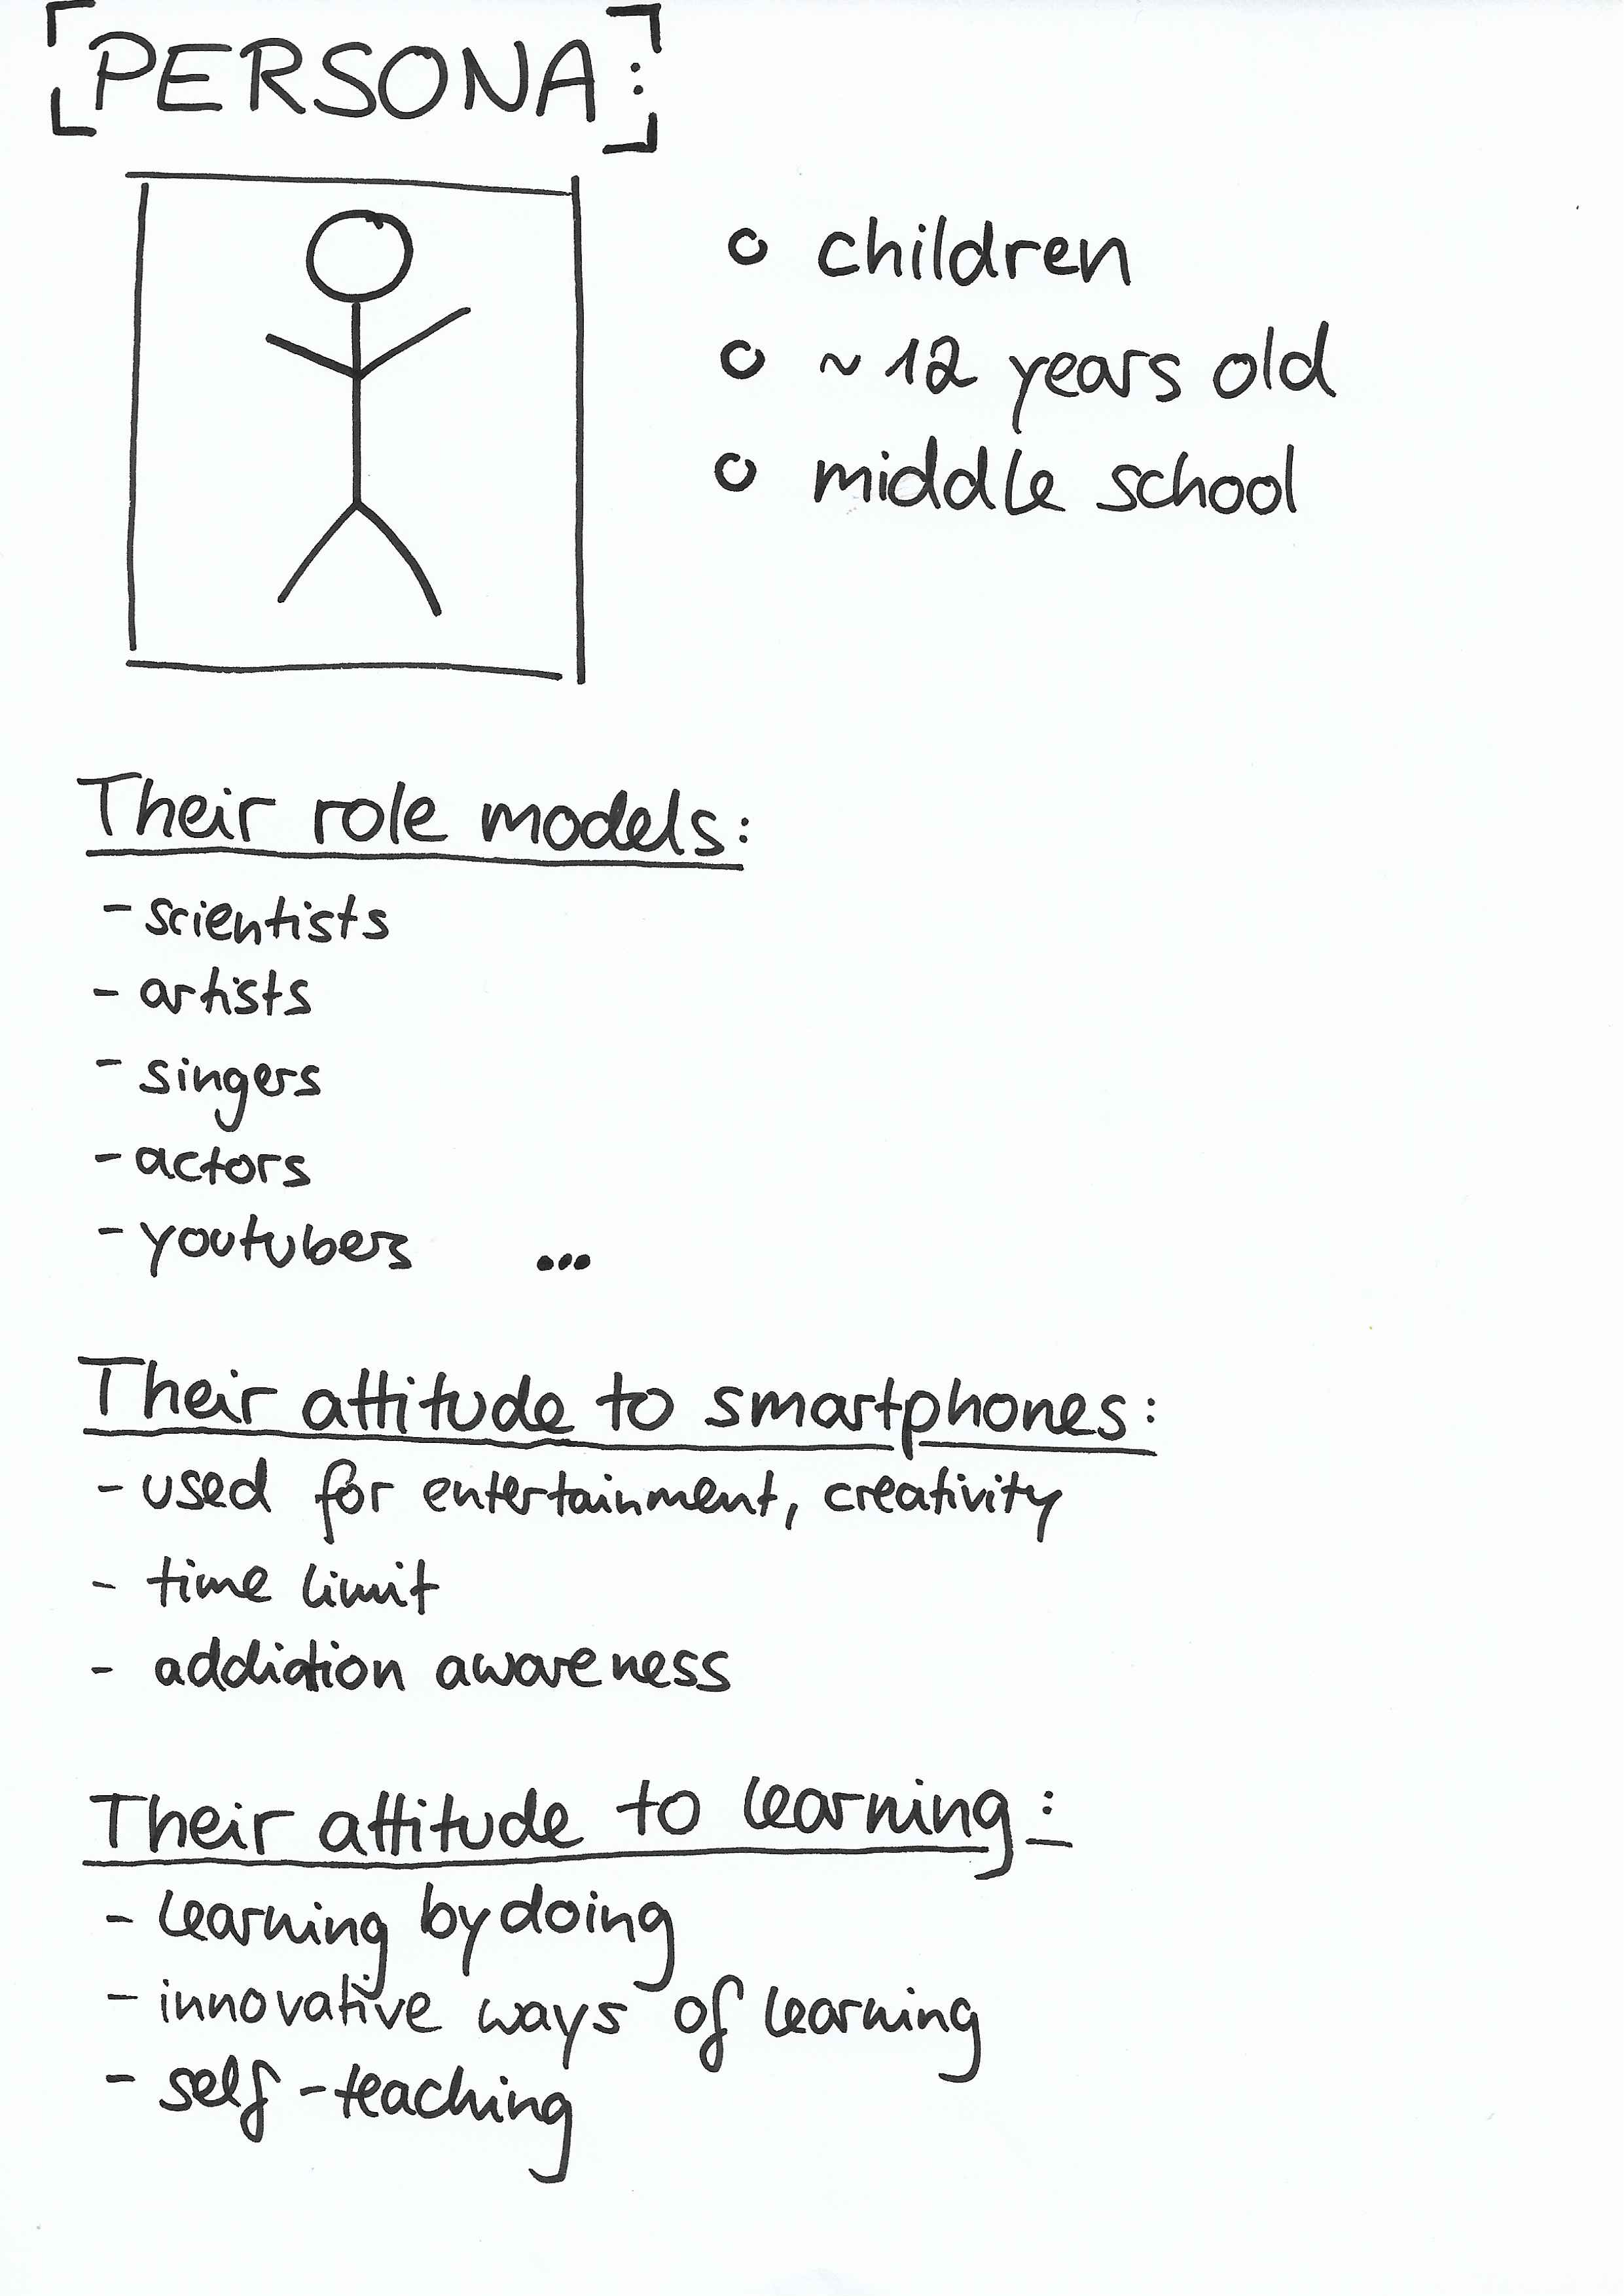
\includegraphics[width=\textwidth]{../images/persona.jpg}
       		\caption{Our persona draft}
        		\label{persona1}
	\end{figure}
	

\section{Ideation and sketching}

	Describe your ideation and sketching process and how these two activities fit together.
	

\section{Workspace and materials}

	Describe your workspace and the materials you used.
	
	
\section{Photos}

	If appropriate, show photos of your team at work.
	
	%Kathrin's group picture here
	
	\begin{figure}[H]
        		\centering
       		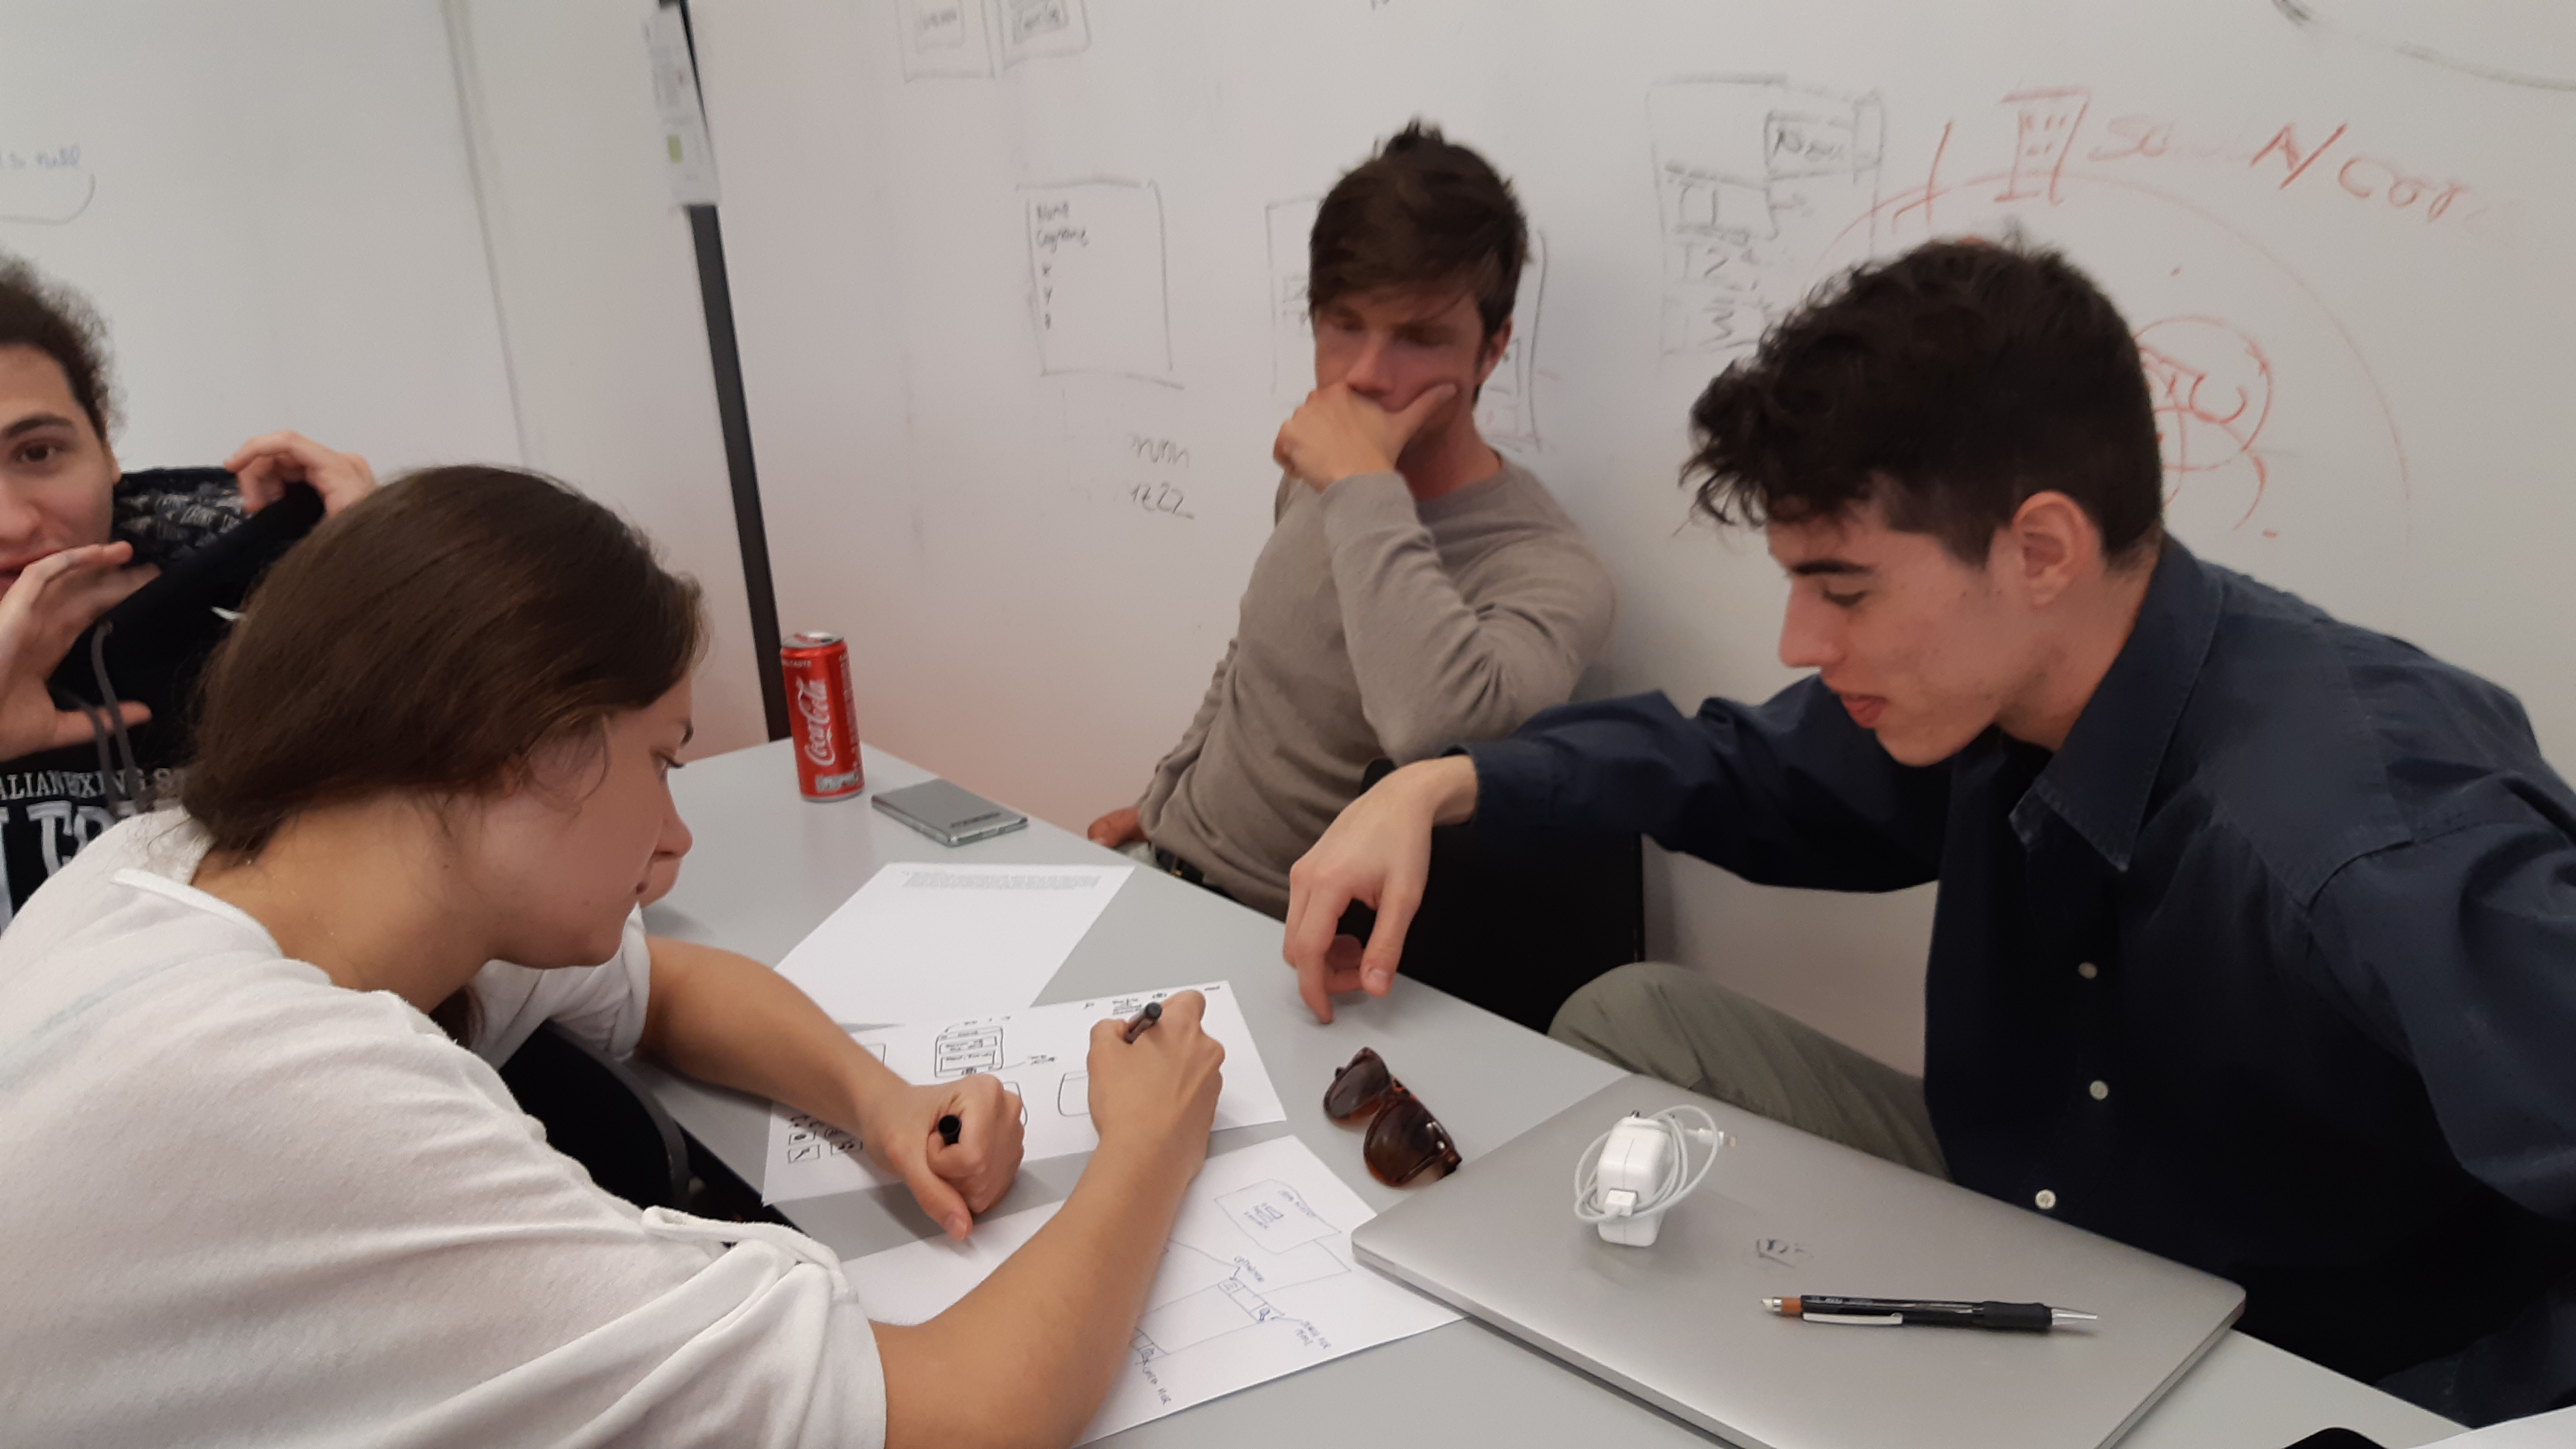
\includegraphics[width=\textwidth]{../images/group2.jpg}
       		\caption{Our team at work}
        		\label{group2}
	\end{figure}
	
	
\section{Sketches}
	
	Show scans of selected sketches.
	
	\begin{figure}[H]
        		\centering
       		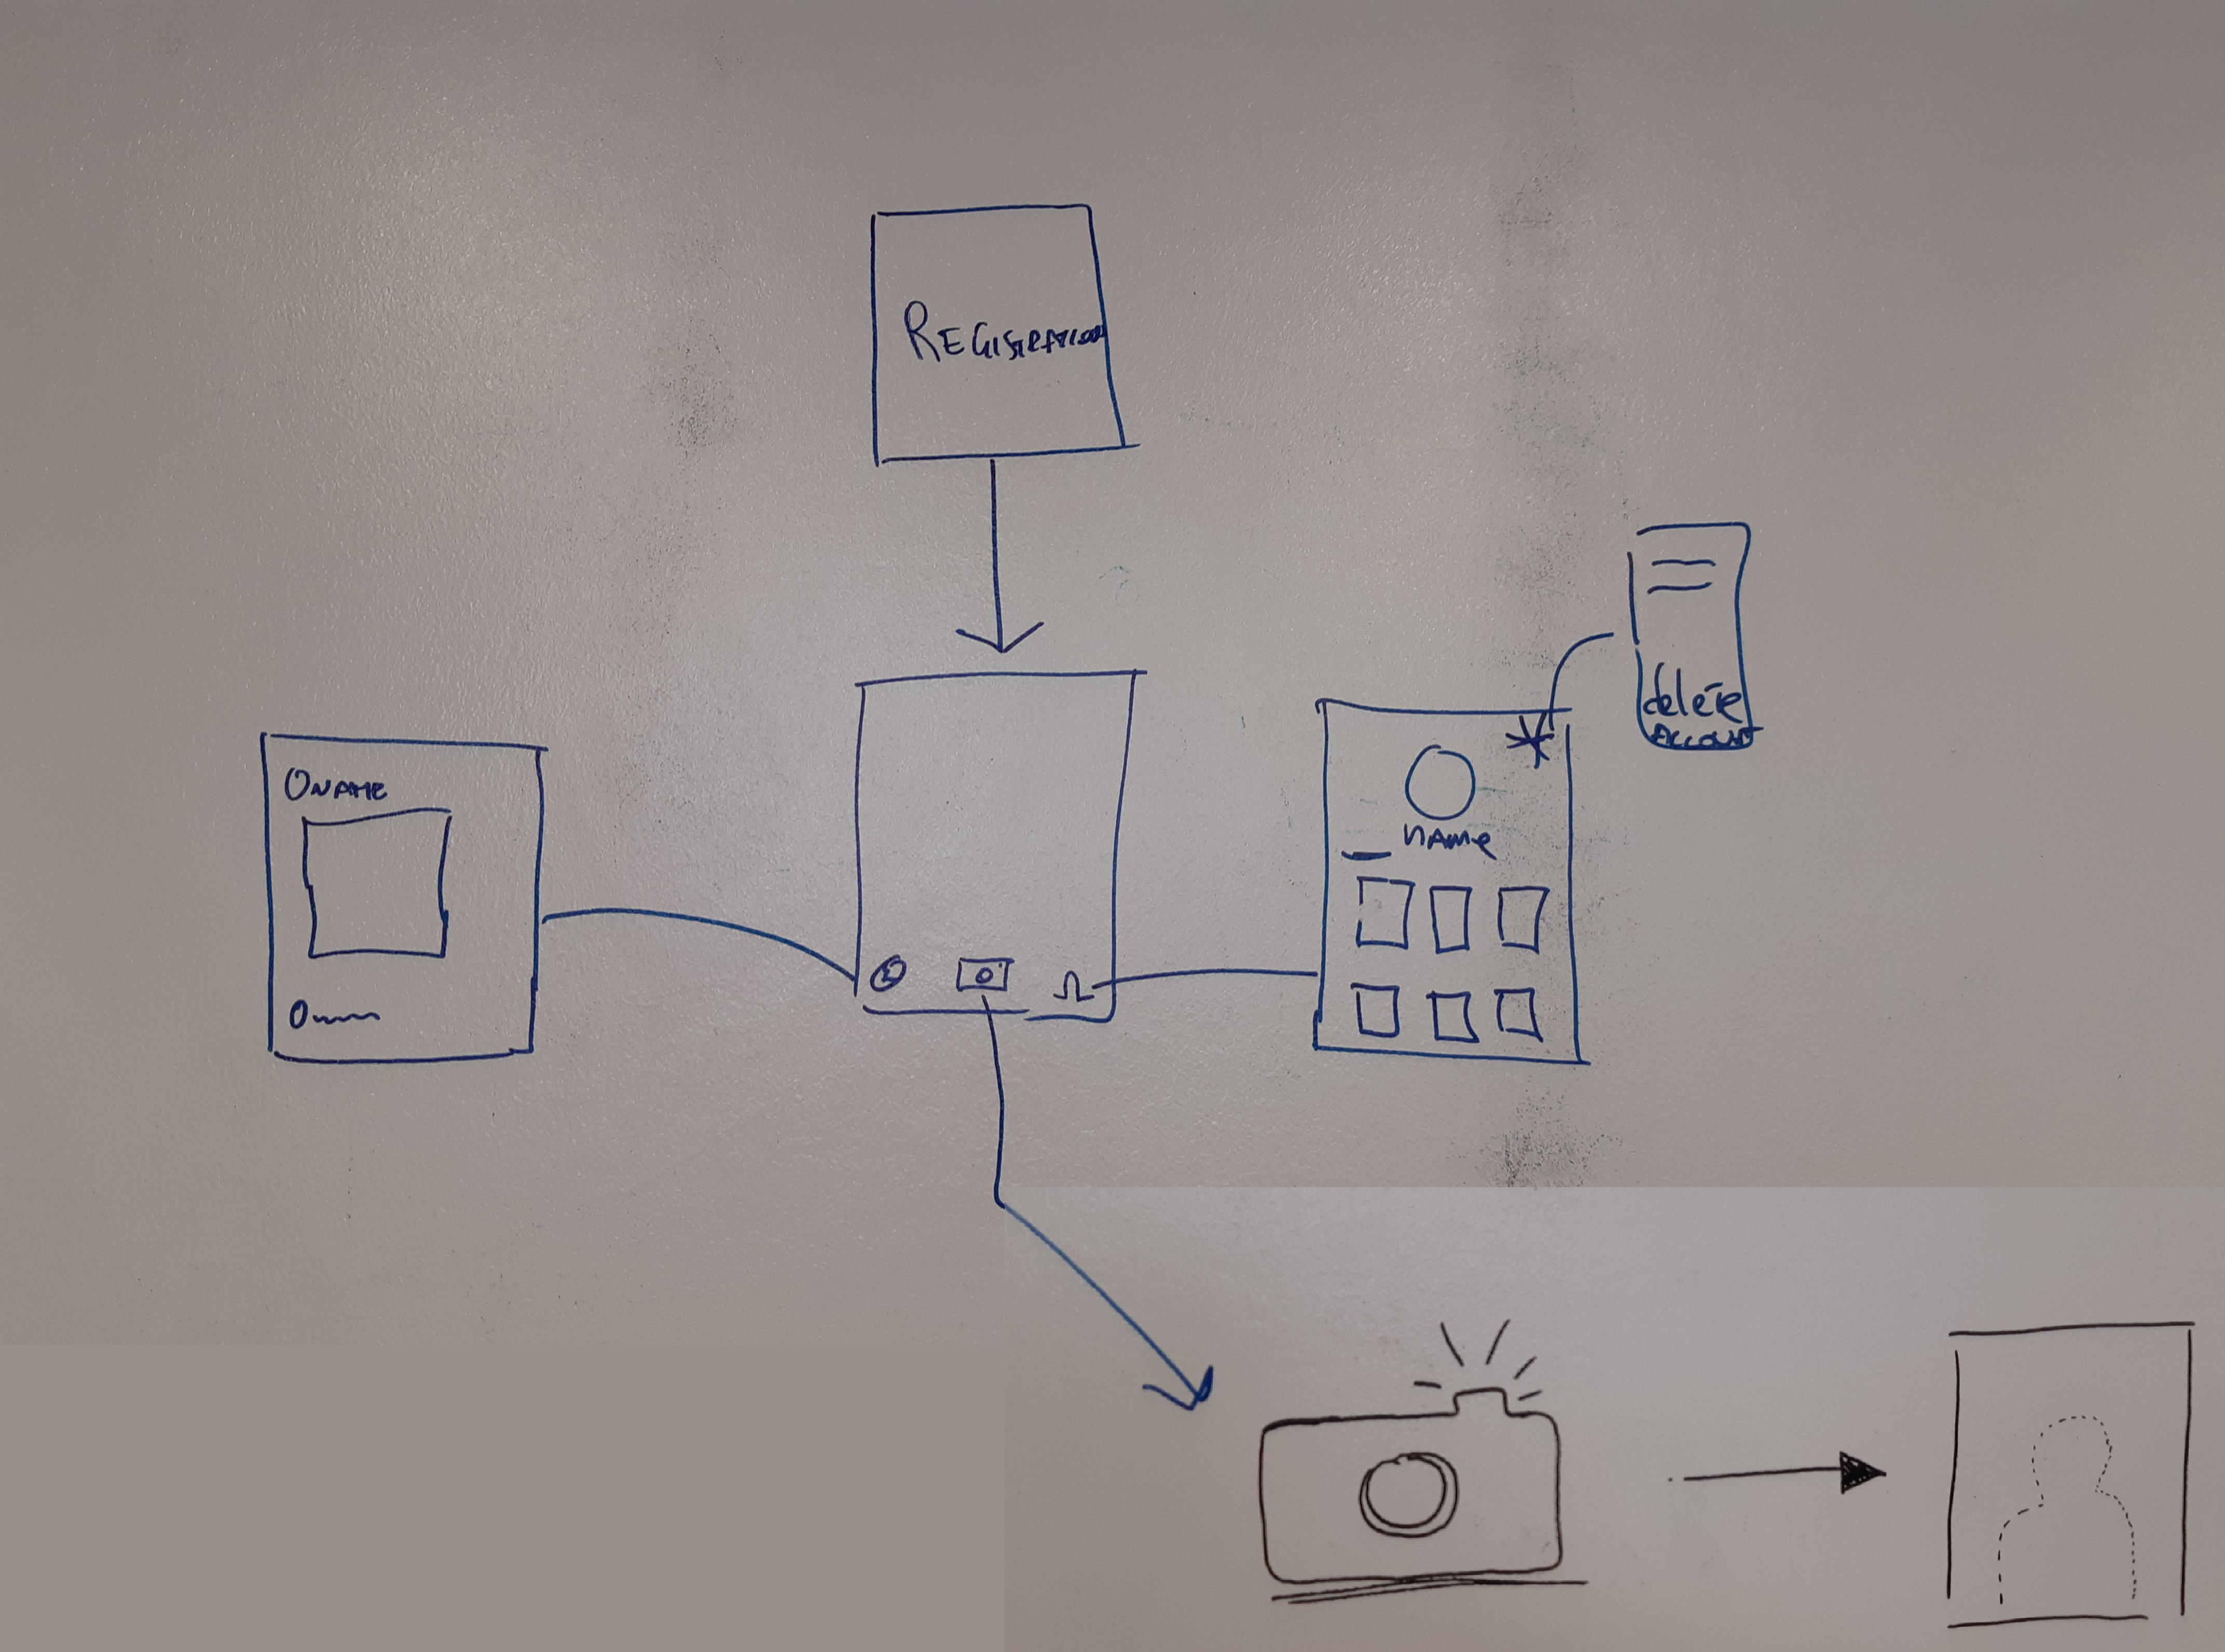
\includegraphics[width=\textwidth]{../images/design1.jpg}
       		\caption{The very first sketch}
        		\label{sketch1}
	\end{figure}
	
	\begin{figure}[H]
        		\centering
       		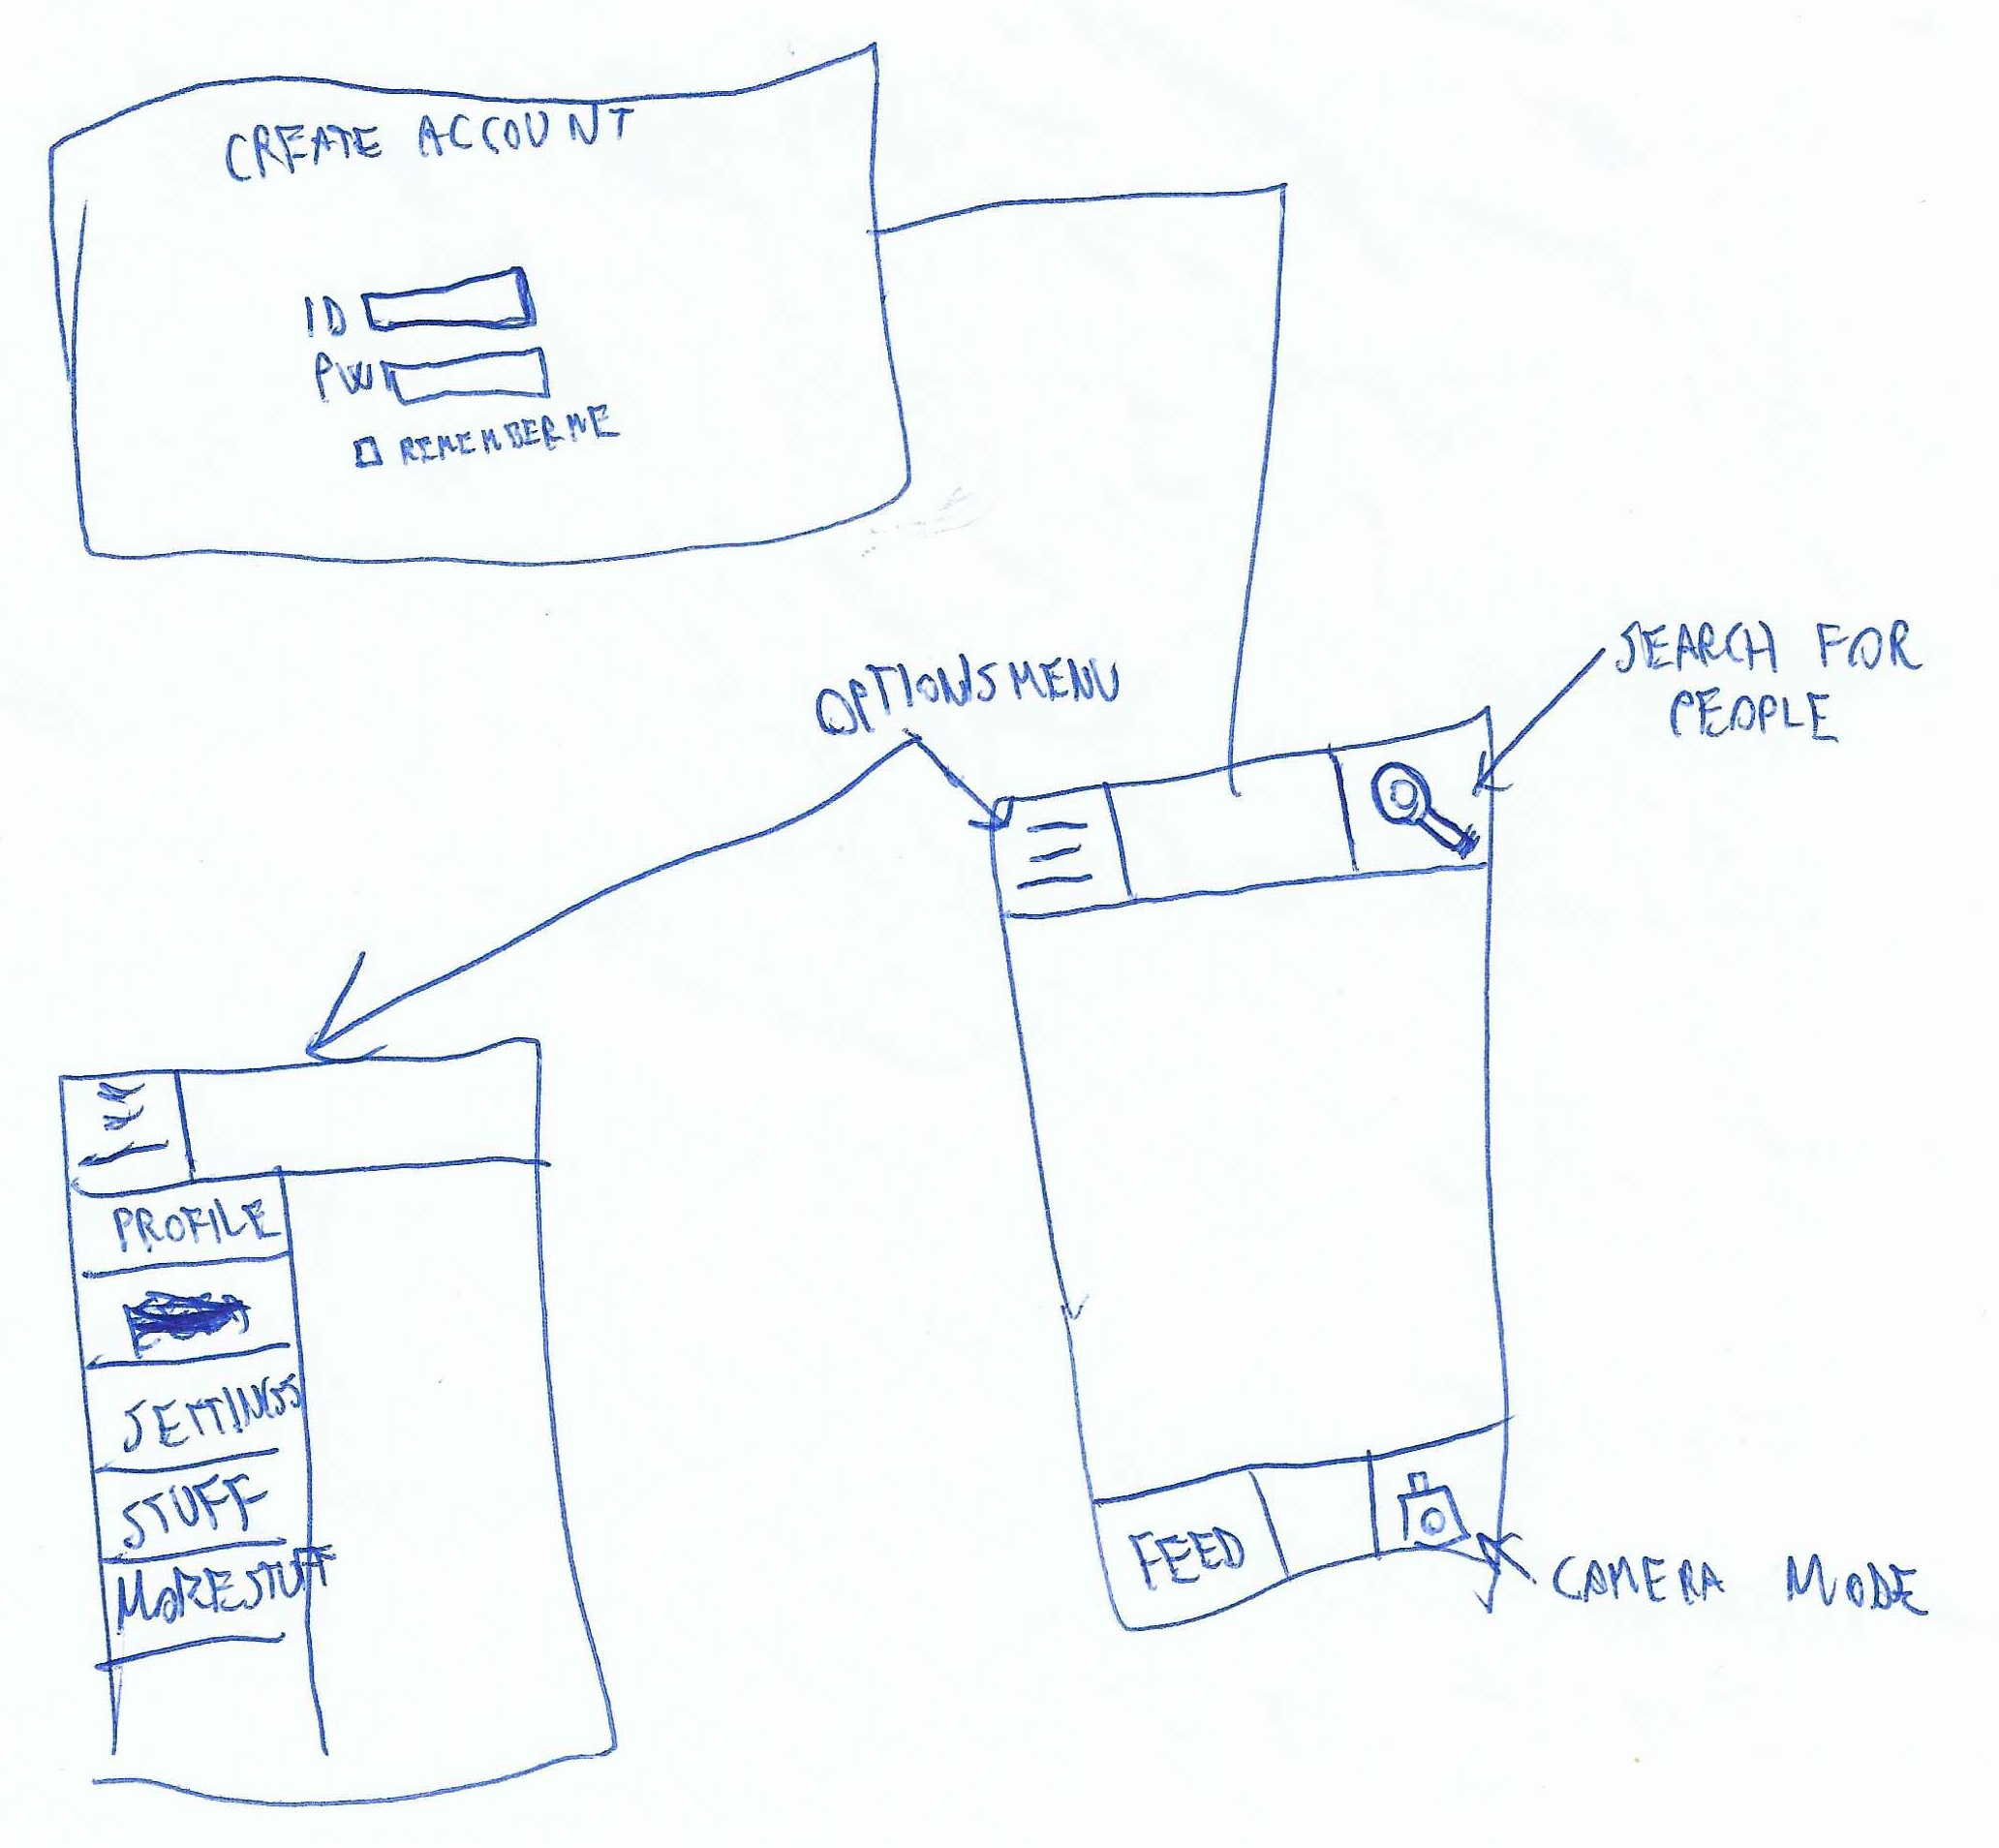
\includegraphics[width=\textwidth]{../images/design2.jpg}
       		\caption{The basic idea}
        		\label{sketch2}
	\end{figure}
	
	\begin{figure}[H]
        		\centering
       		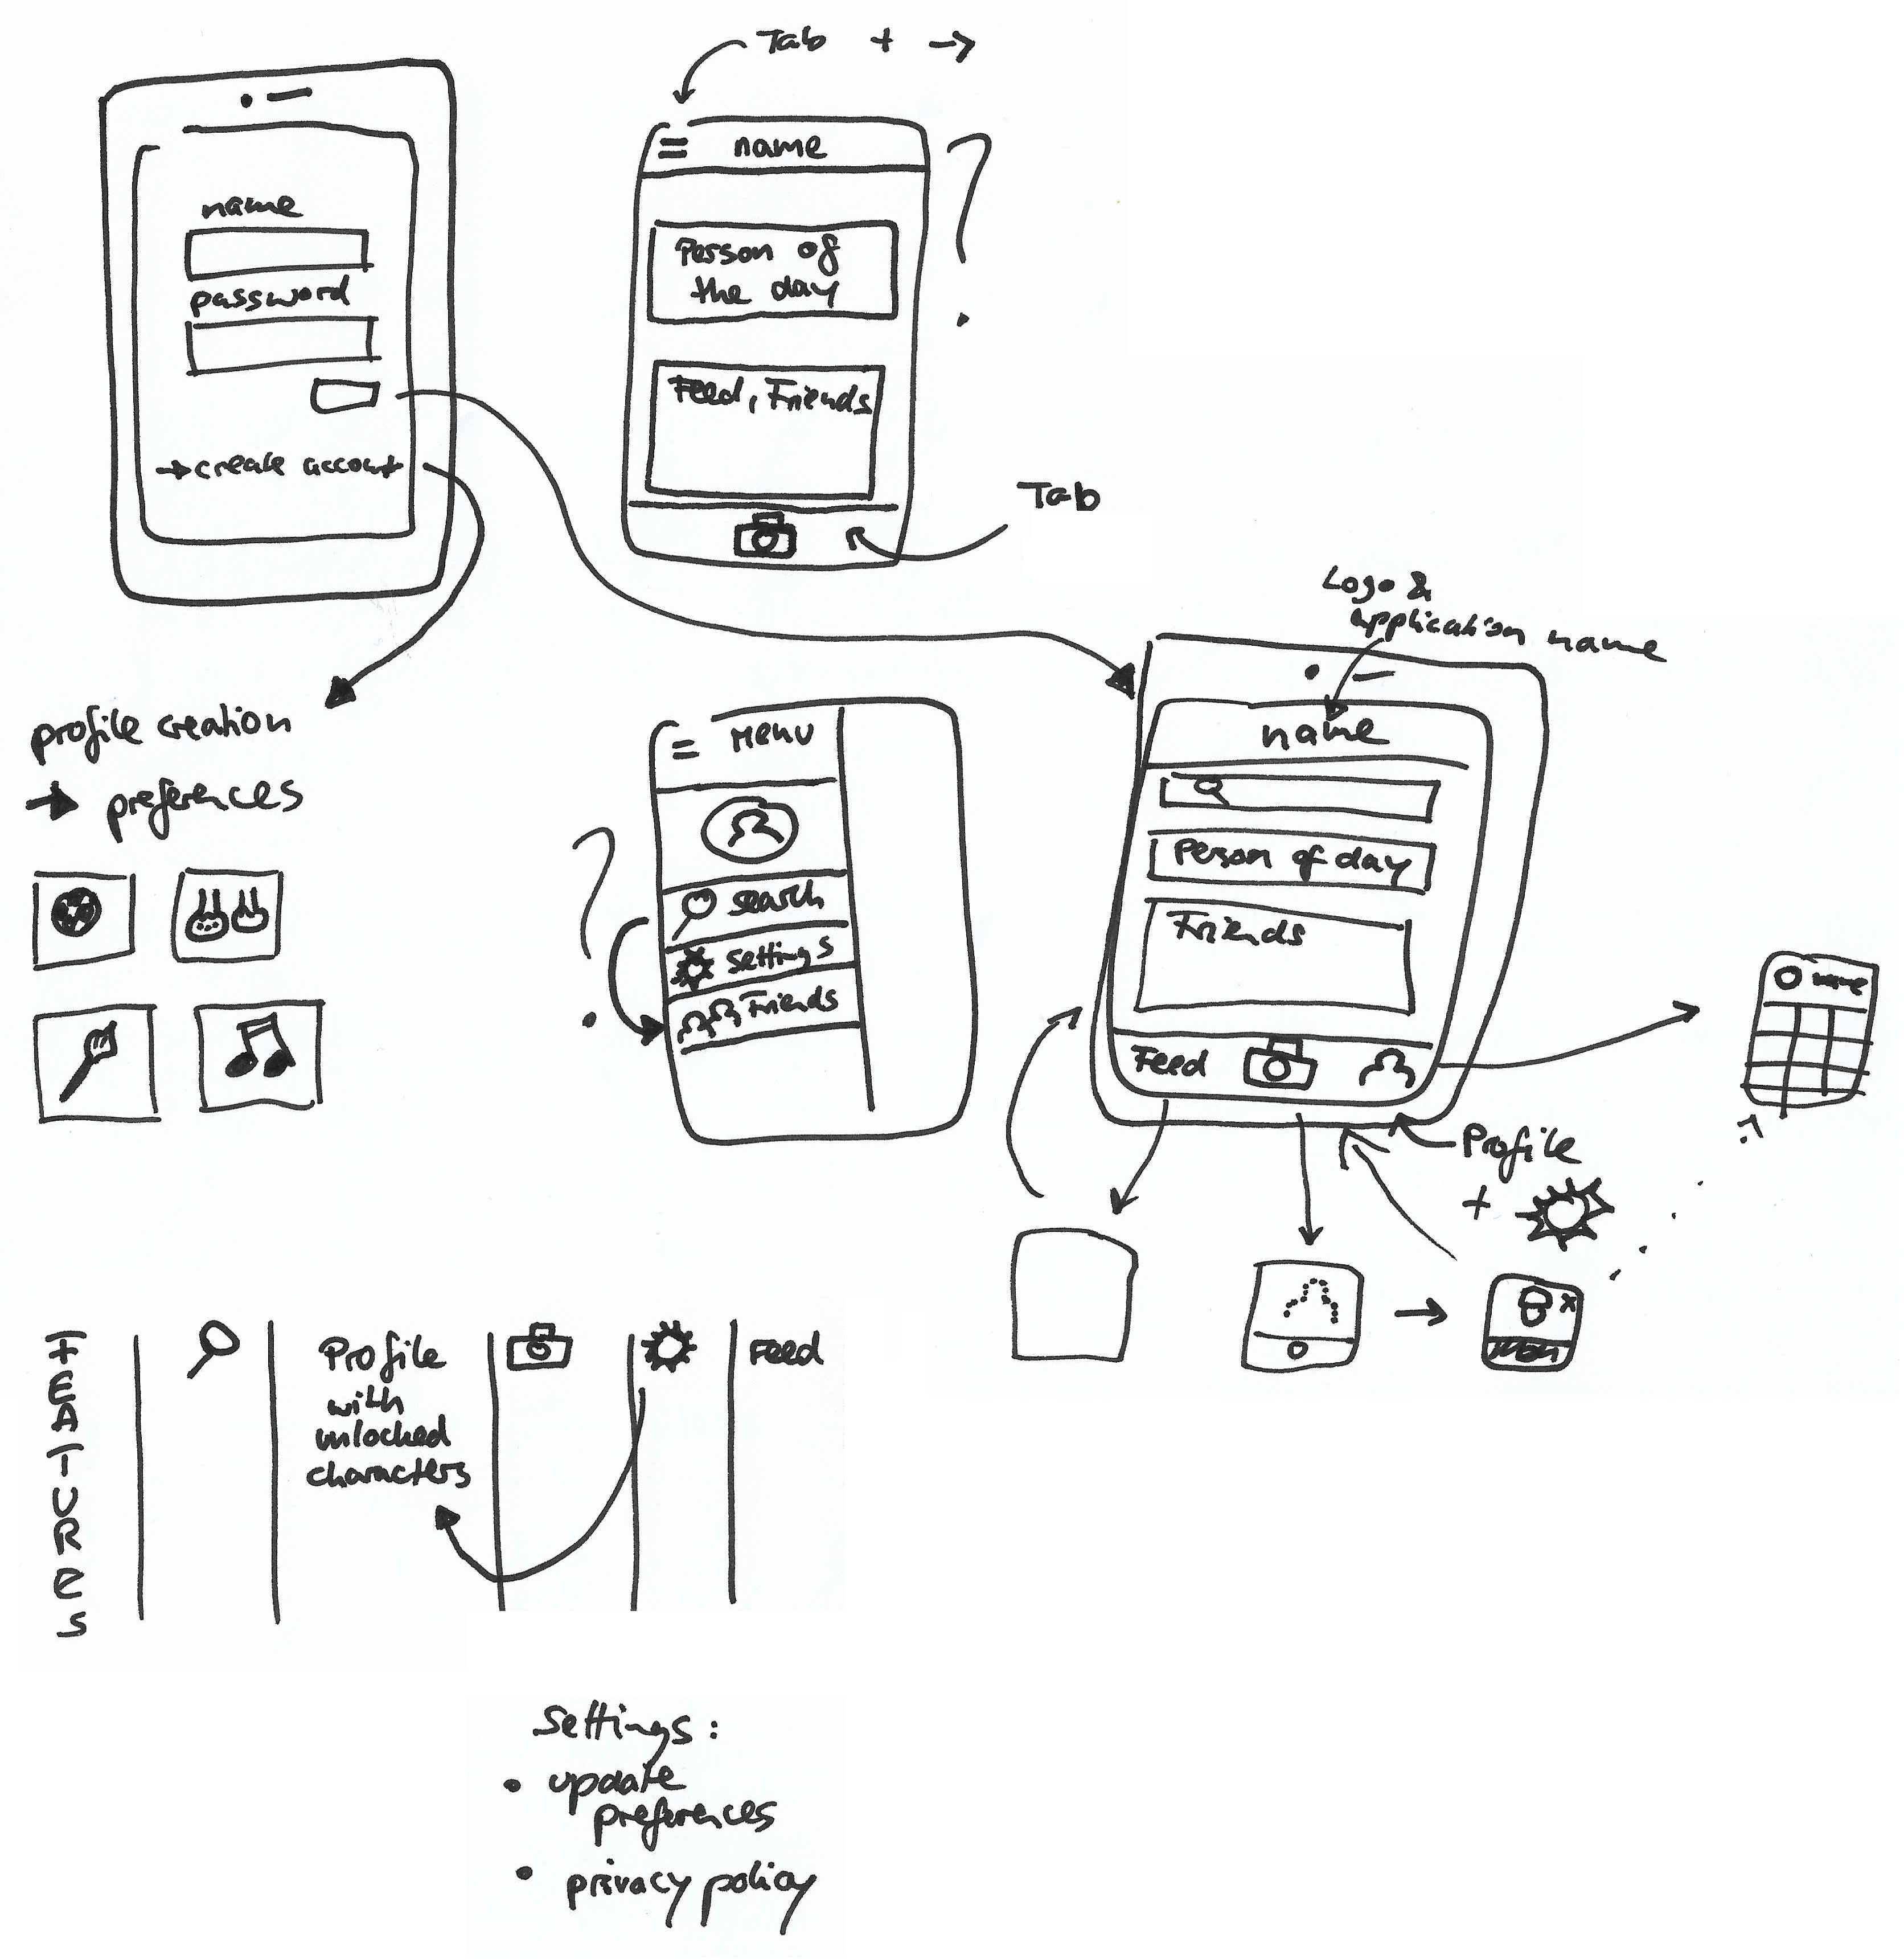
\includegraphics[width=\textwidth]{../images/design3.jpg}
       		\caption{Adding complexity}
        		\label{sketch3}
	\end{figure}
	
	
\section{Storyboard}
	
	Show your storyboard (probably as scans or photos), and explain the process very briefly. Explain the frame that shows the transition from one adjacent frame to another.
	
	\begin{figure}[H]
        		\centering
       		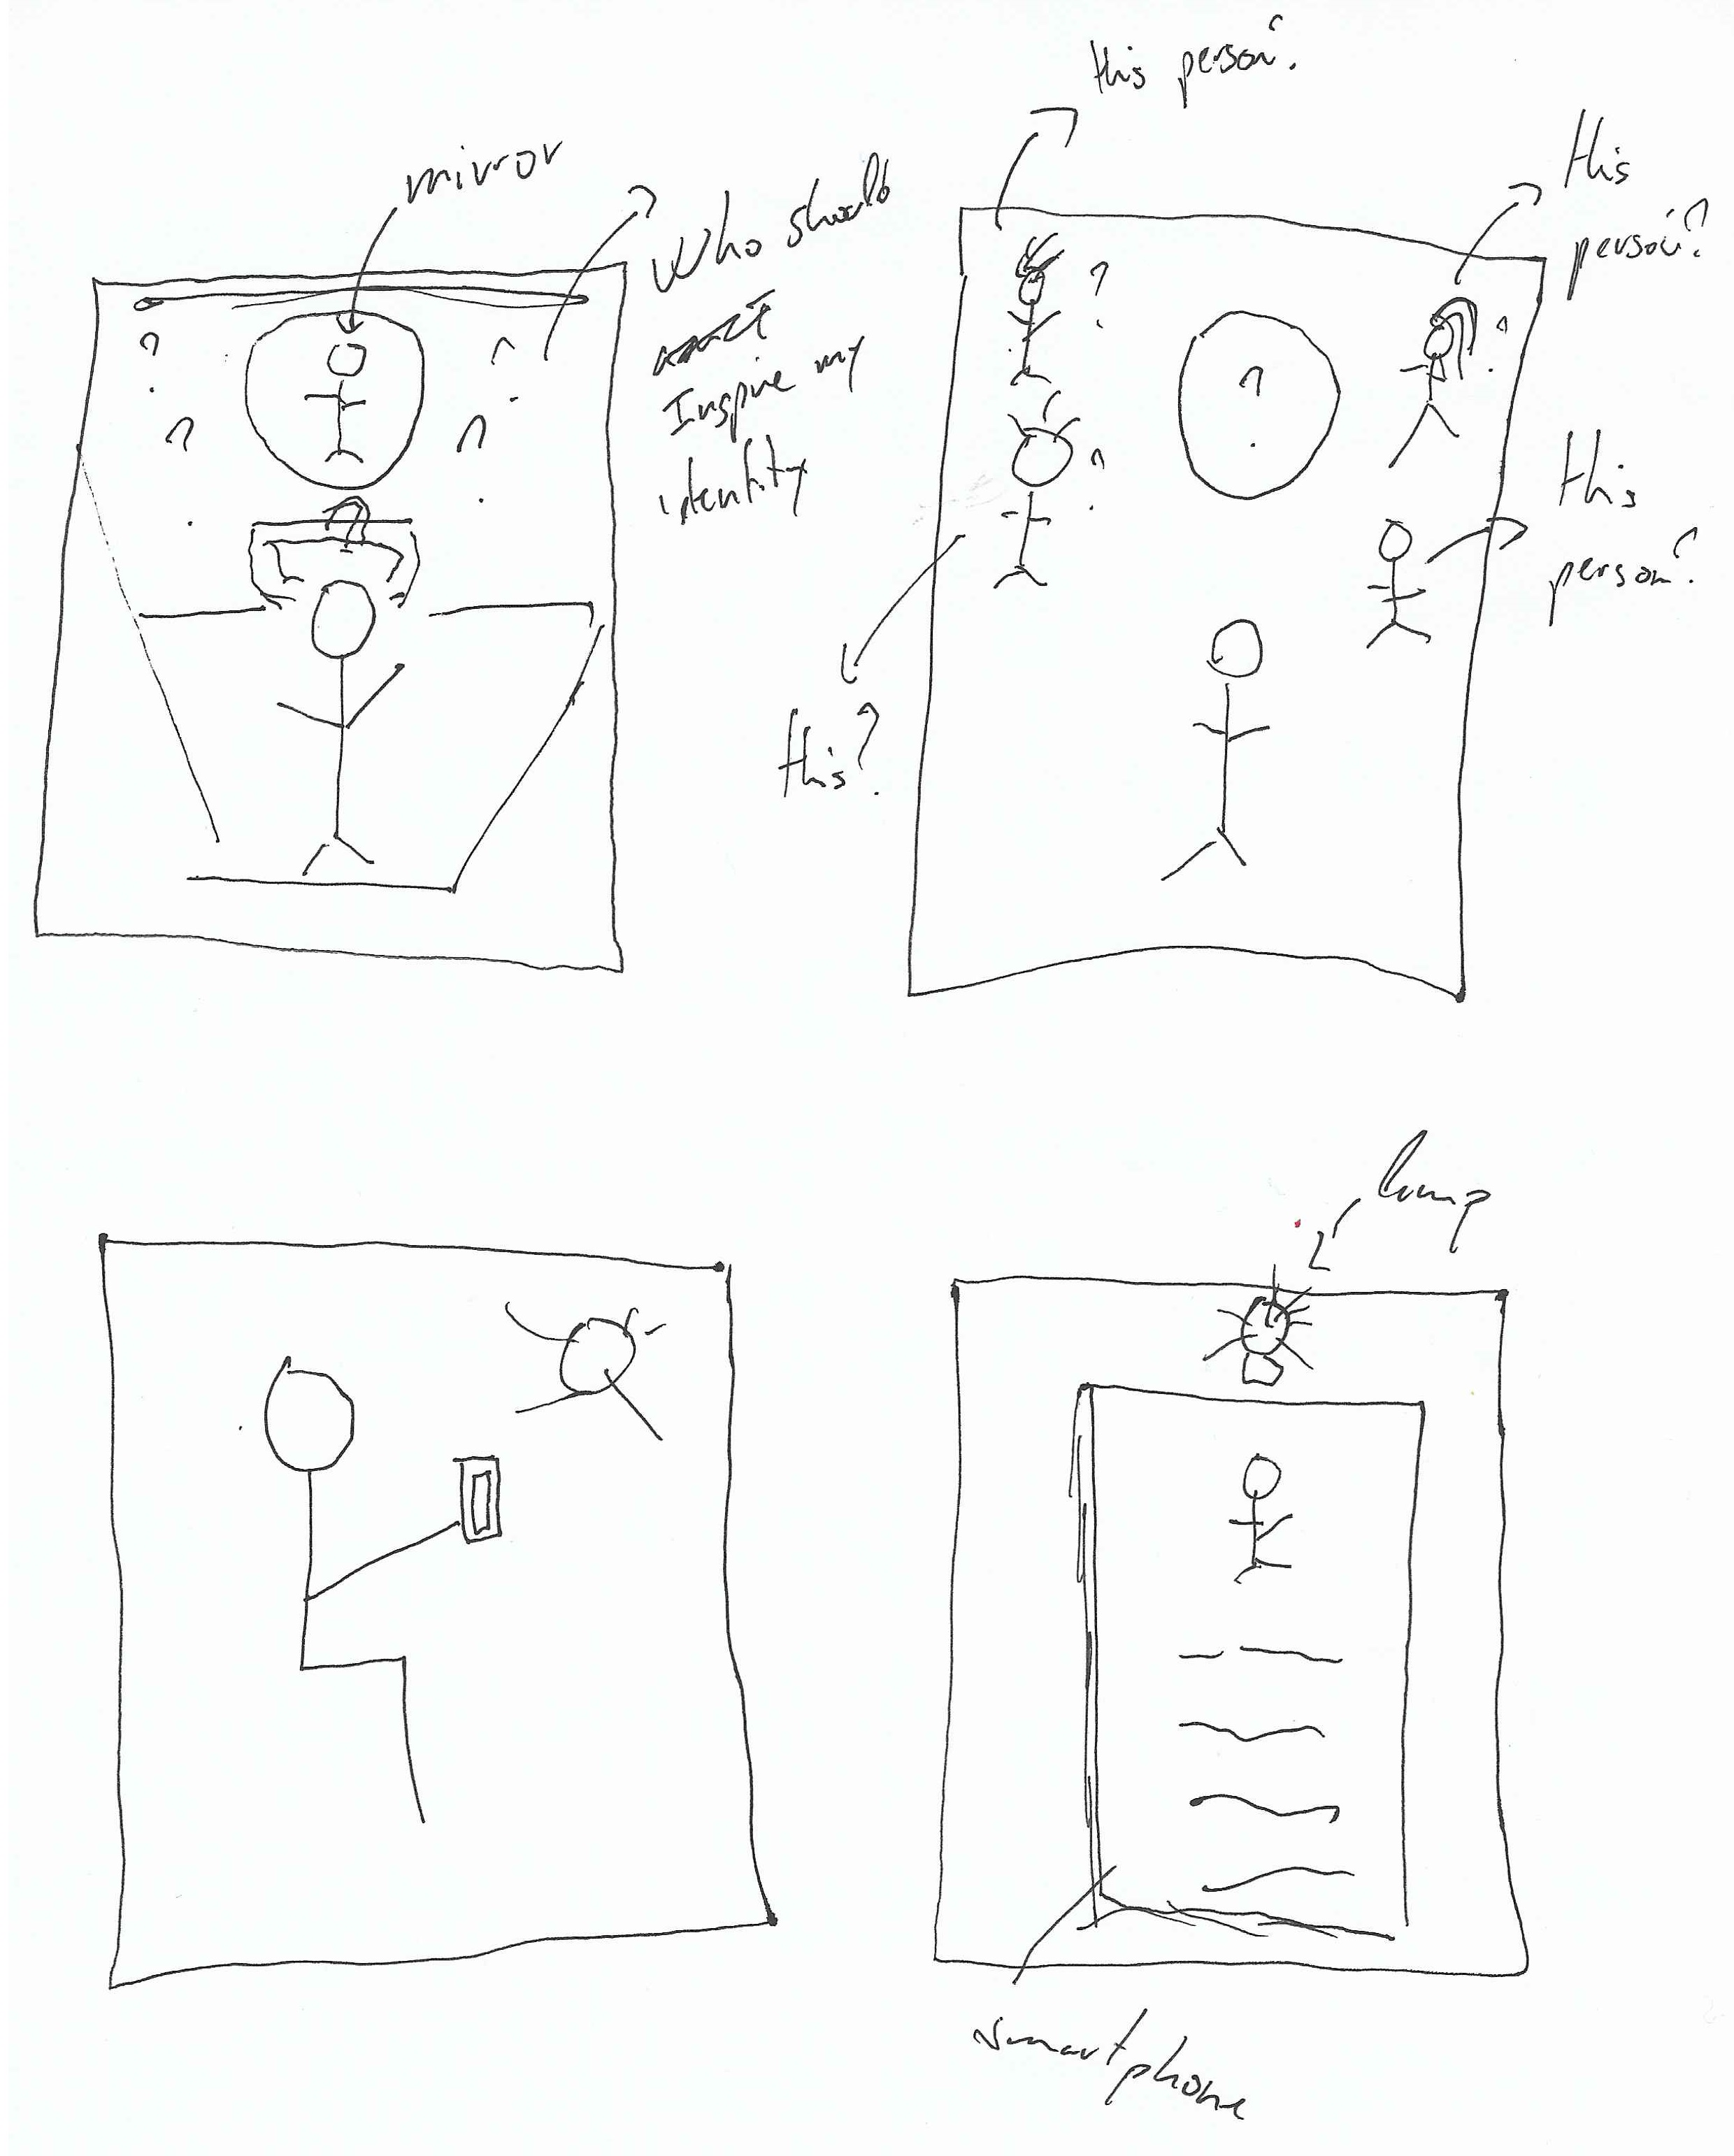
\includegraphics[width=\textwidth]{../images/story1.jpg}
       		\caption{The First Story (by Filippo)}
        		\label{story1}
	\end{figure}
	
	\begin{figure}[H]
        		\centering
       		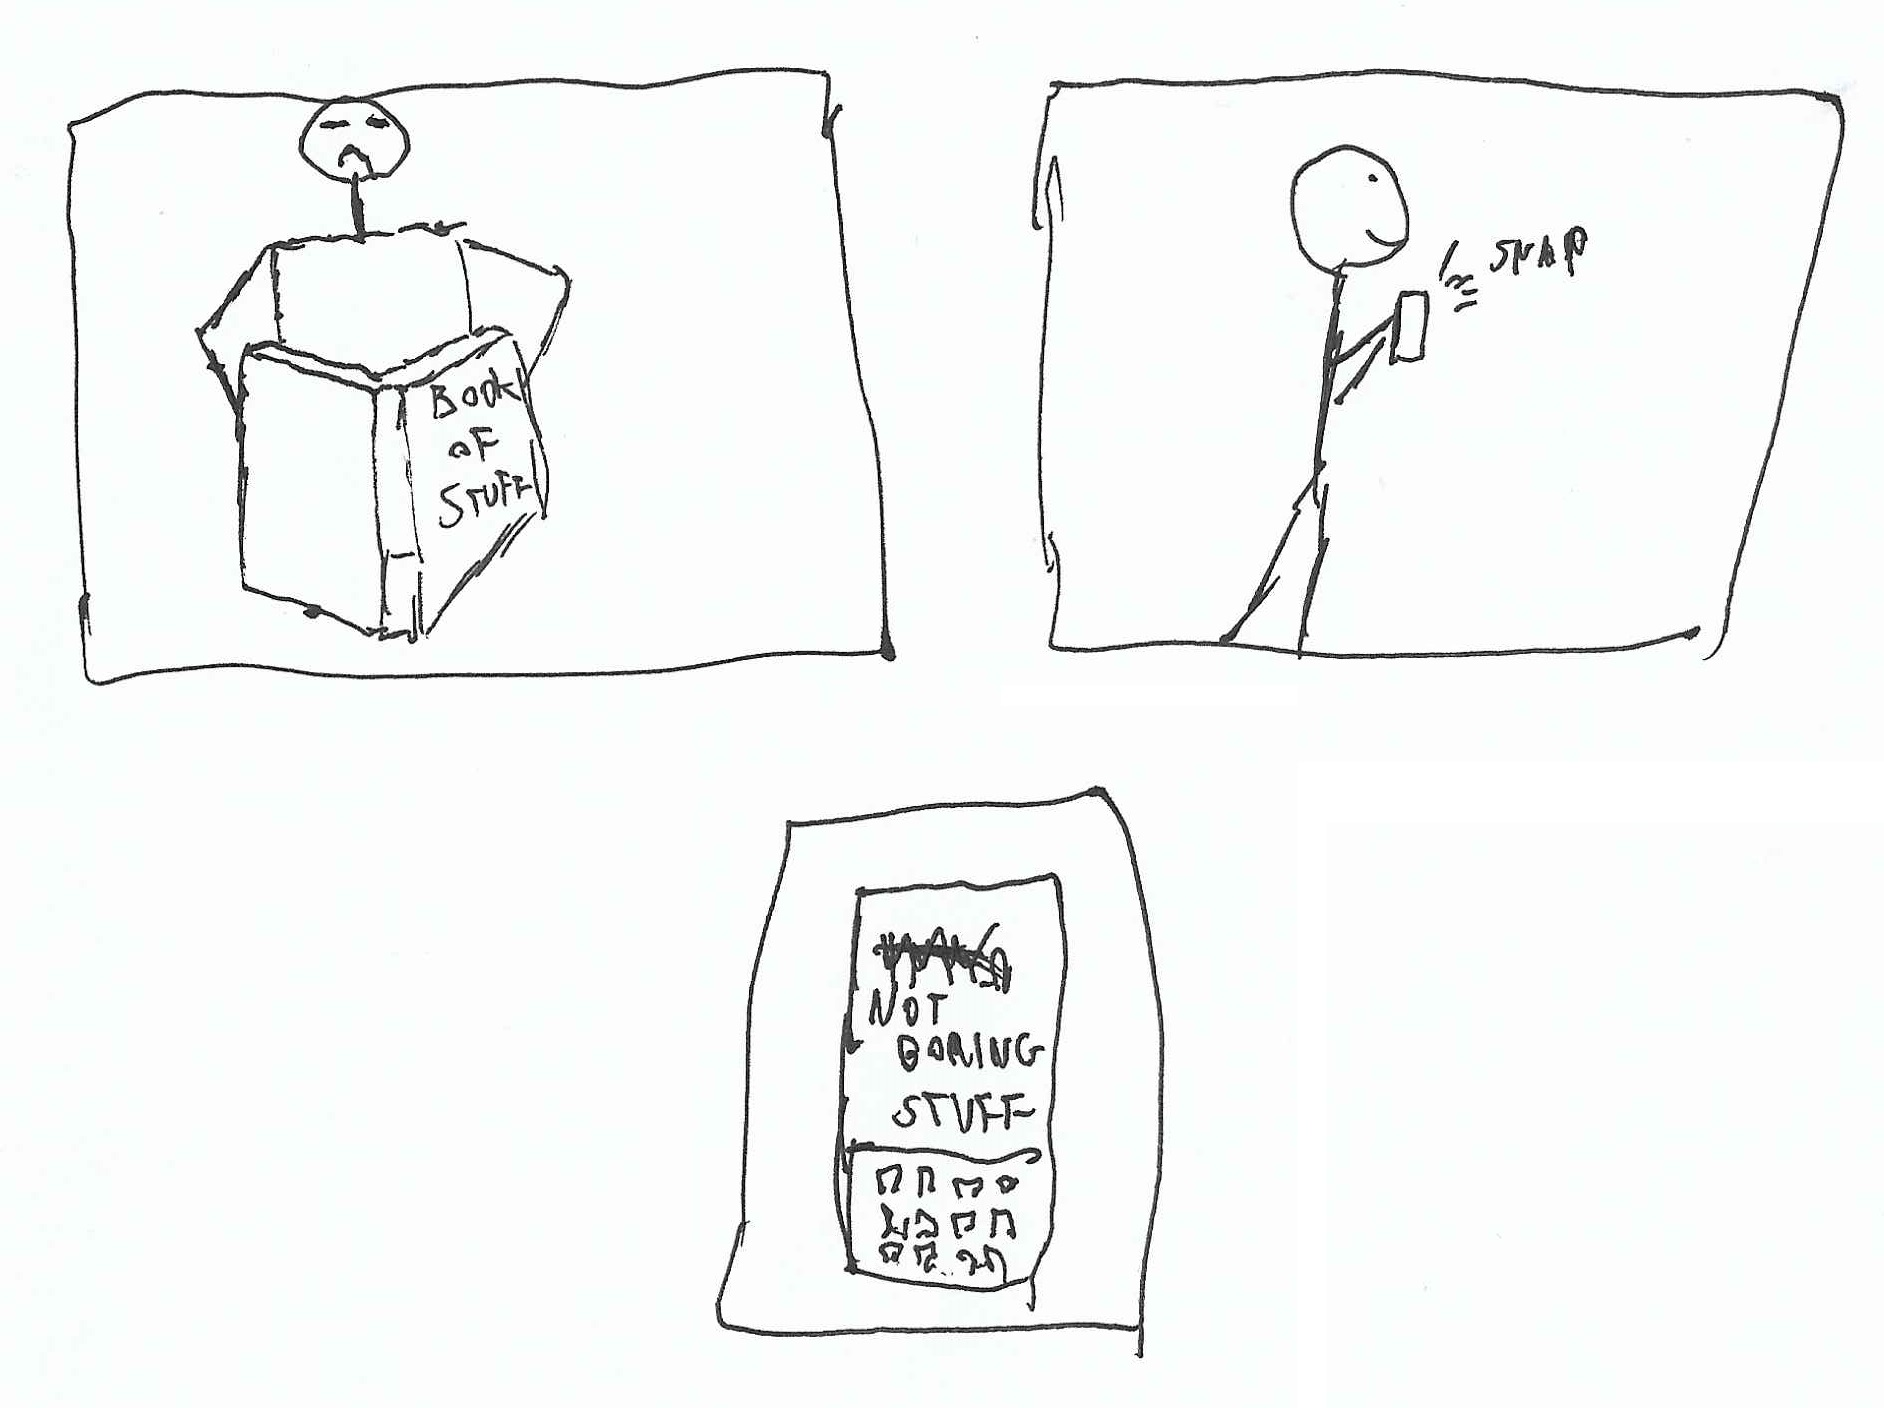
\includegraphics[width=\textwidth]{../images/story2.jpg}
       		\caption{The Second Story (by Tommaso)}
        		\label{story2}
	\end{figure}
	
	\begin{figure}[H]
        		\centering
       		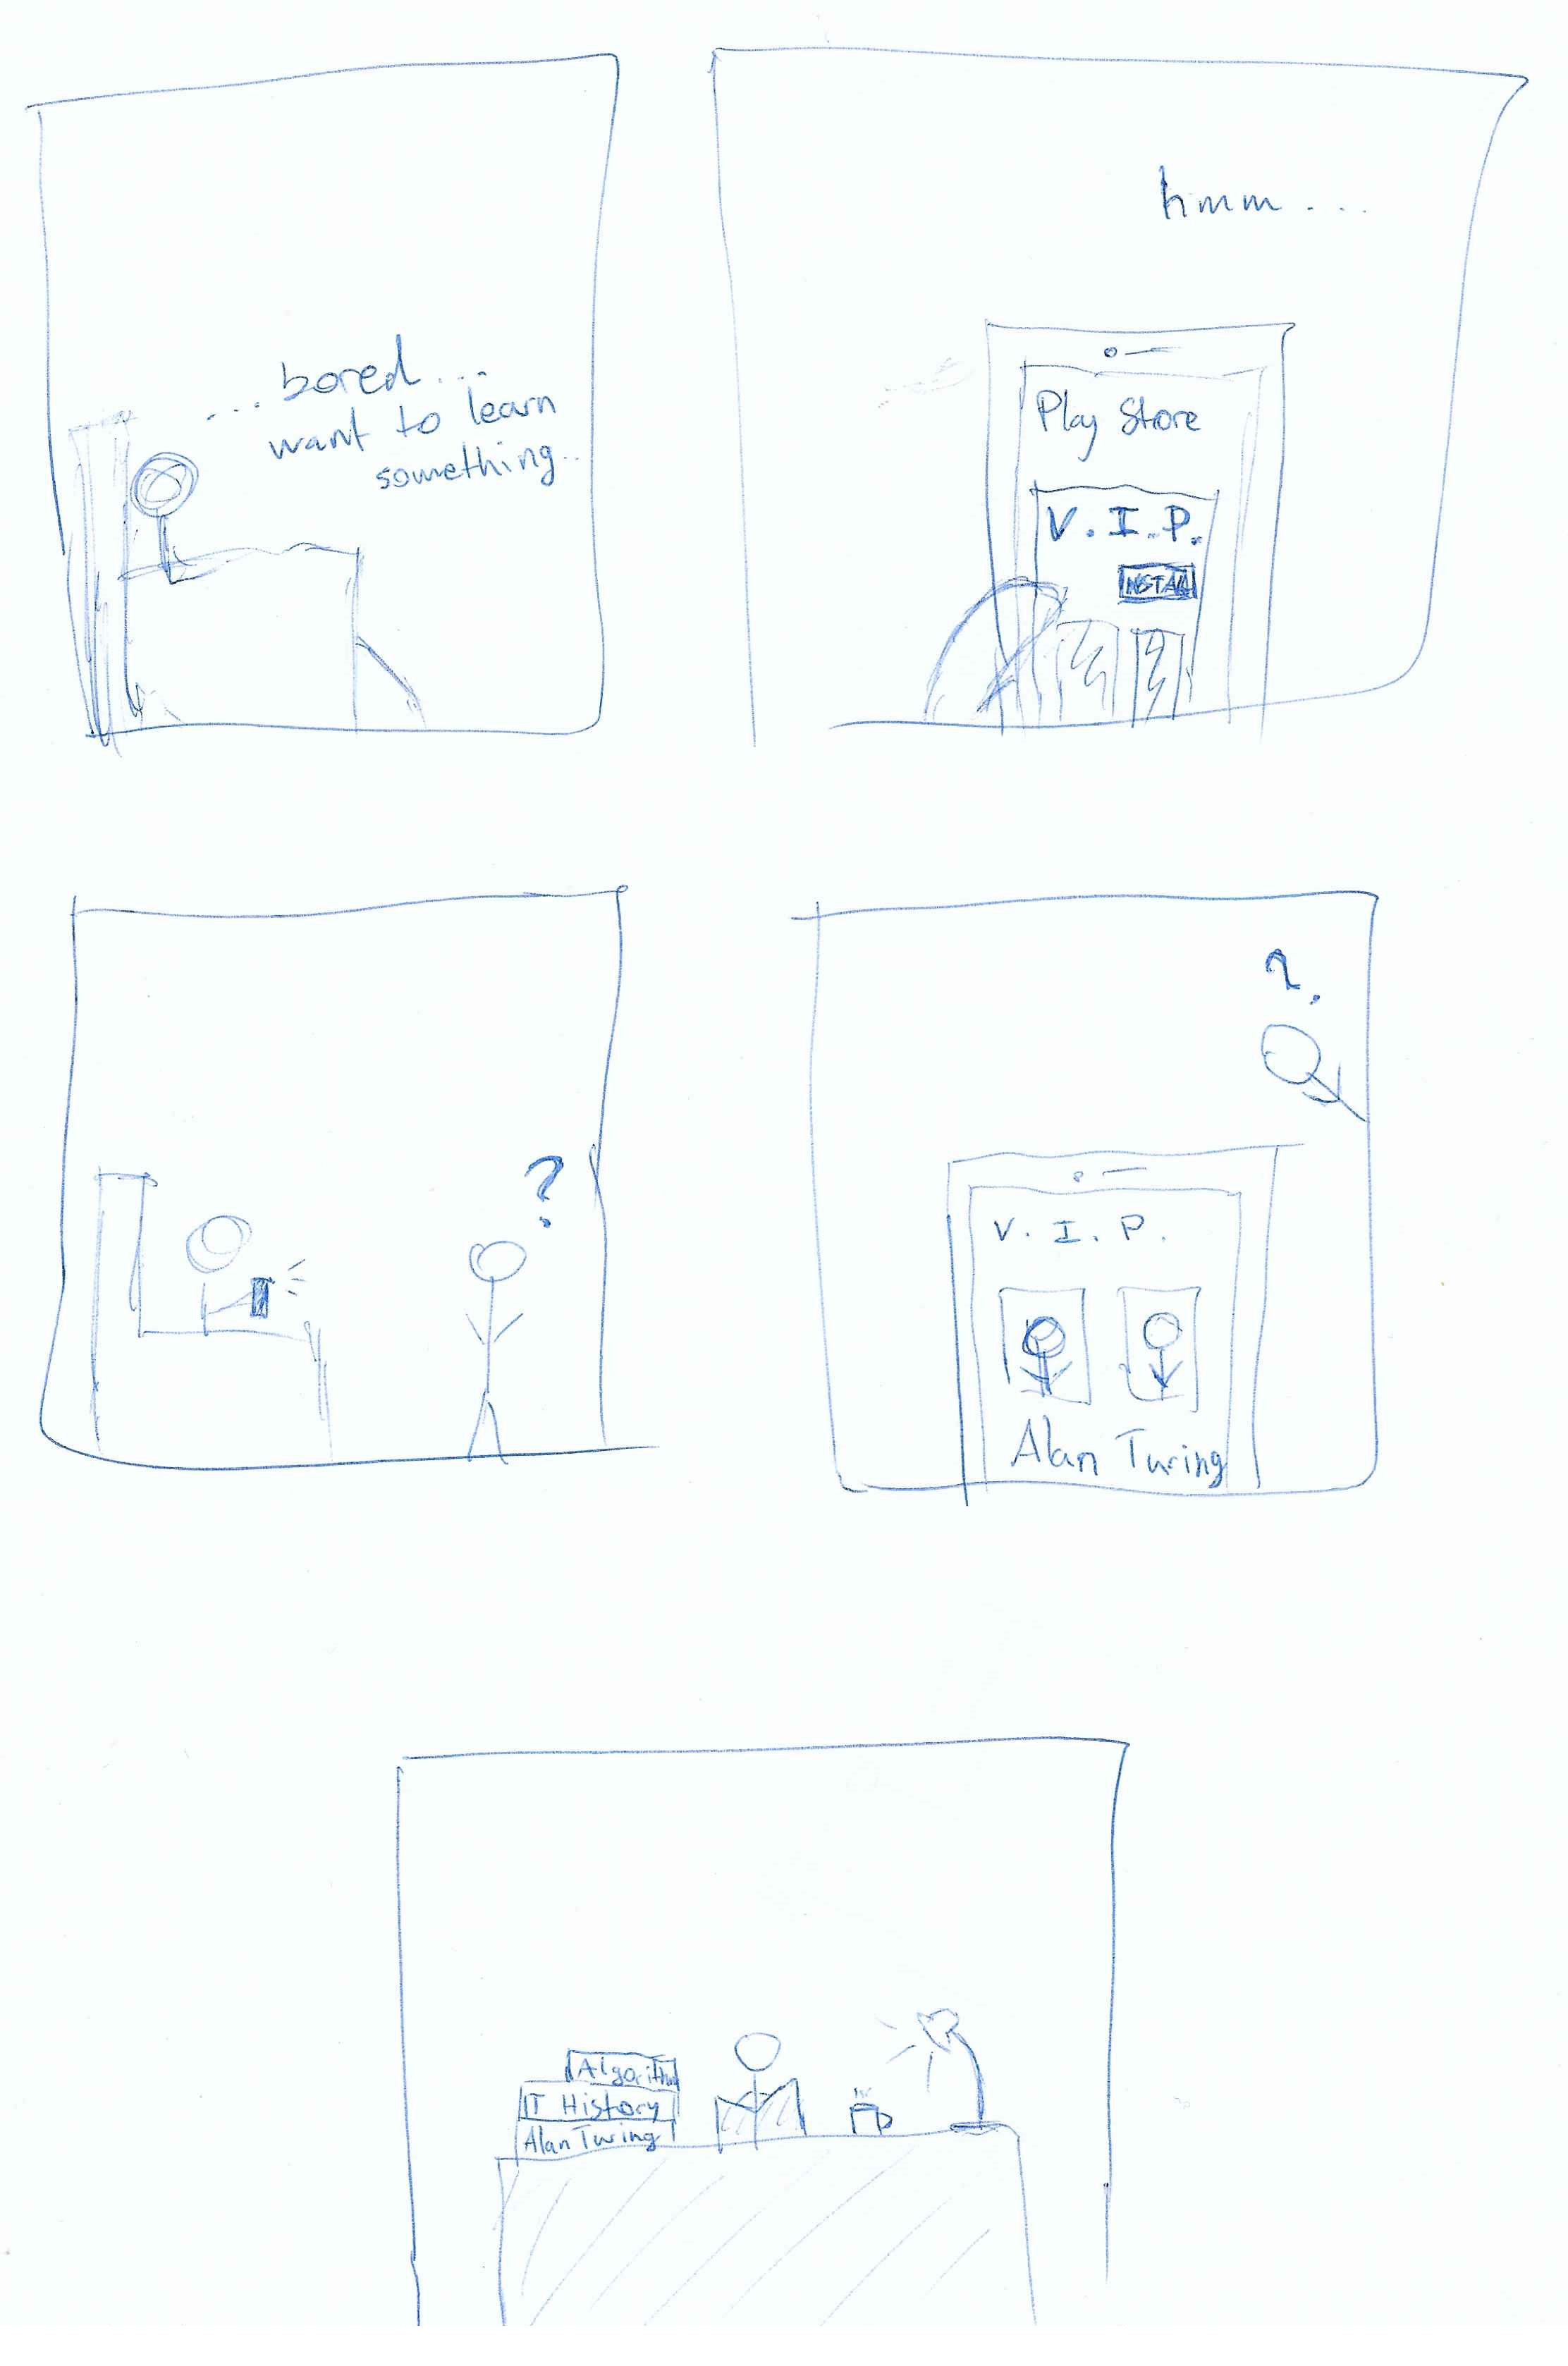
\includegraphics[width=\textwidth]{../images/story3.jpg}
       		\caption{The Third Story (by Stefano)}
        		\label{story3}
	\end{figure}
	
	%Jacopo' story here
	

\section{Wireframe}

	Make a wireframe representation of a set of related intermediate screen designs, corresponding to the usage/design scenario you used for the storyboard above.  Show screen layout and navigation.
	
	%Balsamiq exports?
	
	
\section{Conclusions}

	Write conclusions about what you have learned and progress in your project.
	

\end{document}